\chapter{Ultra-Short Baseline System} \label{chap:proposed_sys}

This chapter is dedicated to the presentation and overall explanation of the developed system, highlighting its capabilities, the used methodologies and overall design strategies. 
The system will be presented in two distinct sections. The first component is the HDL module, which falls into the spectrum of hardware design and requires insight on hardware development and good practices. The second section relies on software development to complement the functionality of the mentioned module, so that is possible to deliver the desired result.

\section{HDL Module Architecture} \label{subchap:HDL module}

The system which is proposed to be implemented in this research work has as input 4 signals which are received by each hydrophone of the array, and outputs an average phase difference between all combinations of pairs of hydrophones. 

\note{
- regras basicas de hardware development\\
- sistema sincrono, available clock cycles globais\\
- hardware limitations\\
- tamanho das entradas
arg}


\begin{enumerate}
	\item Hilbert Filter
	\item Cordic
	\item phasediff
	\item phasemean
\end{enumerate}

\subsection{Module components}

apresentar esquema global menos pormenorizado

\subsubsection{Hilbert Filter}

\begin{eqnarray}
H(f)(t) = \frac{1}{\pi}\int_{-\infty}^{\infty}\frac{f(\tau)}{t-\tau}d\tau
\label{eq:hilbert_integral}
\end{eqnarray}

\begin{eqnarray}
&Imag_0 = x_{-1}*c_1 + x_{-3}*c_3 + x_{-5}*c_5 + x_{-7}*c_7
\label{eq:hilbert_imeq}
\end{eqnarray}

\begin{eqnarray}
&Real_0 = x_{-4} 
\label{eq:hilbert_reeq}
\end{eqnarray}

\note{
- matematica brevemente, equação base, resposta impulsional, ganho, coeficientes e ordem usada \\
- schematics  \\
- explicar design decisions \\
- descrever brevemente flow do sinal no hardware
}

\subsubsection{Cordic}
\note{
- descriçao do que faz \\
- entradas e saídas, clocks, ROM
}

\subsubsection{phasediff}
\note{
-pequeno esquema \\
- 1 sub
}

\subsubsection{phasemean}
- pequeno esquema \\
- N accumulated \\

\subsection{Analysis}

\note{present used resources\\ overall achievement}


\section{Position Estimator} \label{subsec:AoA}

The proposed position estimator uses vector algebra, the phase differences obtained from the system described in \ref{subchap:HDL module}, synchronization elements and additional mechanisms that will be further explained in the present section.

\subsection{Preliminary considerations}

\subsubsection{Number of sensors}
For the estimation of the position in 3D space, a multilateration approach was used. As explained in \ref{subsec:multilateration}, the concept of multilateration combines the information of the relative distances between multiple sensors and a target in order to locate it. 

In the present case, a total of four sensors are needed so that it is possible to define the position of target. Using only two sensors, two possibility spheres are formed around these sensors whose intersection originates a circle that contains the location possible solutions. By adding a third sensor, this circle is intersected by another sphere which originates only two location possibilities. Finally, a fourth sensor is added so that it is possible to exactly differentiate which one of the two final solutions is the accurate location solution. 

\subsubsection{Phase Ambiguity}

When the information about the time of arrival of a signal is available, it is relatively easy to estimate the range of the communication since there can be a direct conversion between them. However, when dealing with phase differences, there is no exact time notion, so it is necessary to start by defining a reference point. 

Considering sinusoidal signals, when we have an array with four hydrophones spatially placed to form a 3D layout, the signal that is arriving to each  hydrophone in different times consequently have different phases. However, since sinusoidal signals are periodic, this means that for different signal periods the same phase value is observed, i.e. the phase is ambiguous. It is possible to observe this phenomenon in figure \ref{fig:phasediff}. In this illustration, $\alpha$ represents the observable phase difference of hydrophone $H_4$ to the reference point $H_1$. However, the actual phase difference which is intended to obtain, $\Delta p_4$, is one period of the signal, $\lambda$, added to the observable phase $\alpha$.

\begin{figure}[!htbp]
	\centering
	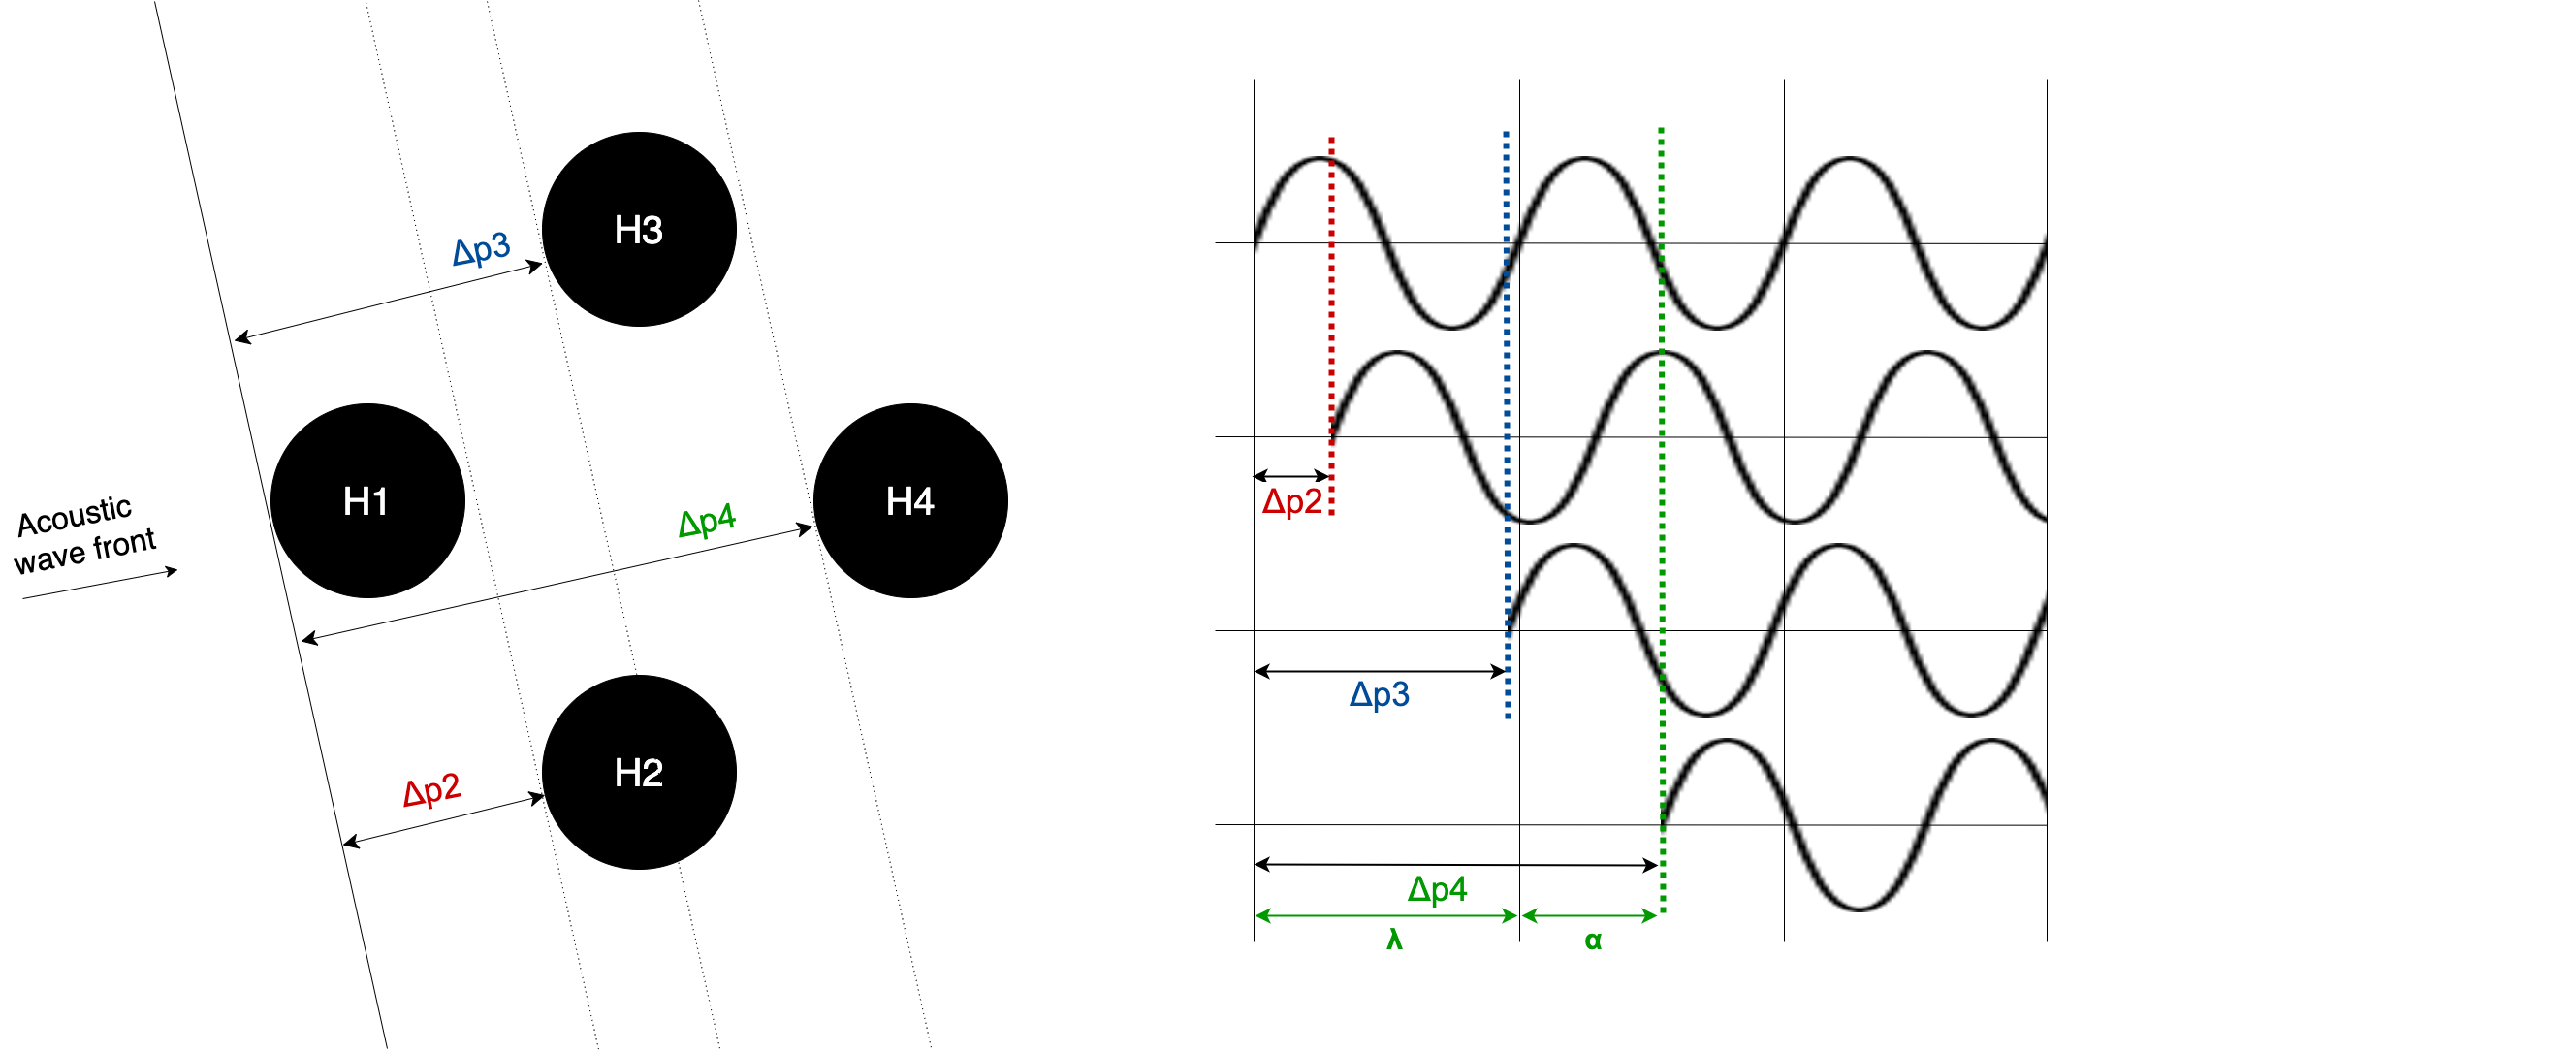
\includegraphics[width=1.2\textwidth]{figures/phase-diff}
	\caption{Phase difference to reference point and phase ambiguity}
	\label{fig:phasediff}
\end{figure}

For this reason, it is crucial to consider that the phase difference is given by the obtained phase value added by the number of periods ahead from the considered reference period.

In the system under study, the sent signals work with a operation frequency of 24.4 $kHz$. The corresponding signal period is $T = \frac{1}{24400} $ seconds which, considering the underwater acoustic speed \textit{c} equal to a standard 1500 $m/s$, the wavelength is approximately equal to $\lambda = \frac{T}{c} = 6.1 cm$. Having this into consideration, after obtaining the time of arrival to each hydrophone given by the cross correlation instances, besides the reference one, it is possible to conclude if the phase shift is superior to one period by analyzing if the time difference is greater than the duration of one period \textit{T}. In figure \ref{fig:phasediff}, each mentioned time difference between $H_1$ and $H_2$, $H_3$ and $H_4$ is converted to the corresponding phase differences $\Delta p_2$, $\Delta p_3$ and $\Delta p_4$.

%From this phase differences, it is possible to estimate the angle of arrival from which the acoustic wave is coming from by comparing all pairs of hydrophones: H1-H2, H1-H3, H1-H4, H2-H3, H2-H4, H3-H4. 

One possibility to solve phase ambiguity in this system would be to place the four hydrophones with a baseline spacing inferior to $\frac{1}{2}$ of a wavelength, since the maximum reached by phase difference is 180 degrees. This way it would be possible to immediately deduce the phase difference since it would always be contained in one period. However, positioning the hydrophones closer together leads to smaller  values,causing a consequent increase on the estimation error due to varying environment conditions (briefly enumerated in \ref{subsec: acoustic-channel}). Additionally, since the hydrophones to be used in this system have a corresponding diameter of roughly half of a wavelength, they would not allow to execute the mentioned configuration and so this possibility will not be contemplated.

In order to compensate this phase ambiguity, a simple relation was developed which allows to calculate the absolute time difference between the moment a signal is received by hydrophone A, $T_A$, and when the same signal is received by a further hydrophone B, $T_B$. Figure \ref{fig:ambiguity} illustrates this association, where the represented sinusoidal waves correspond to the same signal arriving at hydrophones A and B. This correspondence uses the time stamps obtained by the correlation peaks combined with the calculated phase difference, that is determined in parallel, so that the measurement is more accurate. Equation \ref{eq:phase-amb} translates this relation, where $t_1$ and $t_2$ are the correlation peaks obtained from the signal arriving at hydrophone A and B, respectively, and so by rounding for the next integer number the difference between the correlation peaks, $t_2 - t_1$, we will obtain in which period, $T$, of signal in A will the signal in B arrive. Then the measurement is improved by subtracting a phase difference, $\theta_B - \theta_A$, so that the instant in which the signal is detected in hydrophone B can be defined. 

\begin{figure}[!htbp]
	\centering
	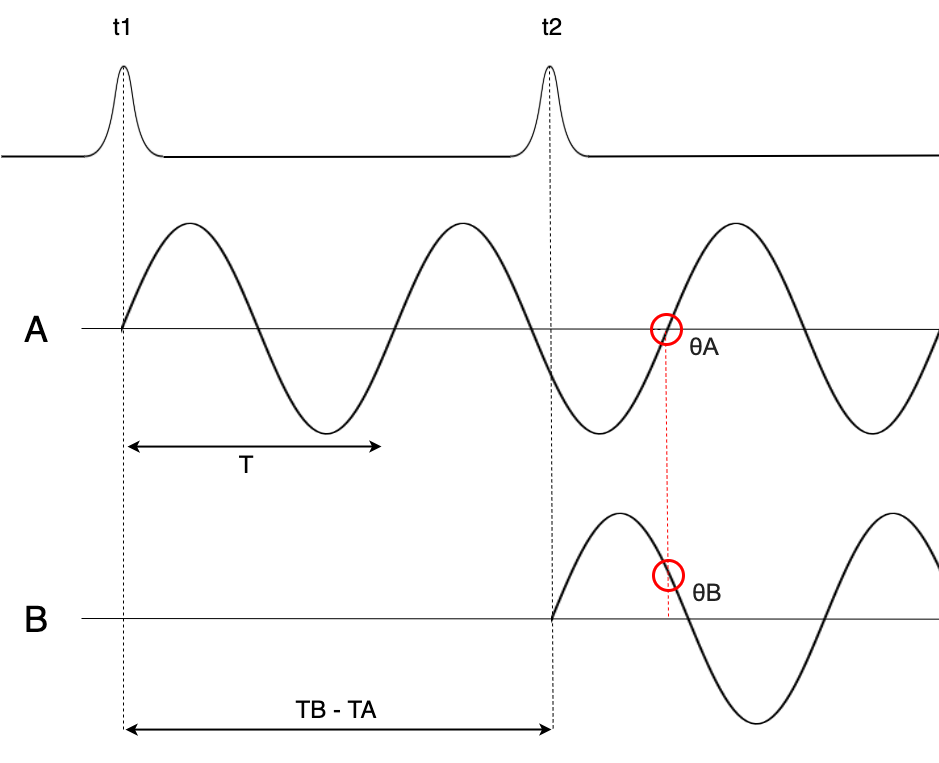
\includegraphics[width=0.6\textwidth]{figures/ambiguity}
	\captionsetup{justification=centering,margin=2cm}
	\caption{Ambiguity correction through correlation and phase difference}
	\label{fig:ambiguity}
\end{figure}

\begin{eqnarray}
& T_B - T_A = round(\frac{t_2-t_1}{T}) - (\theta_B - \theta_A)
\label{eq:phase-amb}
\end{eqnarray}

\subsubsection{Hydrophone position in relation to ToA}
To better understand the location estimation of an acoustic source in relation to the position of a pair of hydrophones, we can initially adopt the two dimensional scenario of figure \ref{fig:hyper}. 

Considering two hydrophones at known relative positions $(-f,0)$ and $(f,0)$, we can model all possible acoustic source locations for a specific ToA through hyperbolas. This is due to the fact that, by definition, the sum of the distances from the focus of each hyperbole, where each hydrophone is placed, to any point of the hyperbolic geometry corresponds to a constant value. 
This means that, in figure \ref{fig:hyper}, any point $(x,y)$ that is contained in the hyperbole corresponds to a constant $|d_2-d_1|$ value which, after some formulation, is in fact equal to $2*v$ or the distance between the vertexes of each hydrophone's hyperbola. Therefore, it is possible to trace a hyperbole that represents the positions of the target in space both based on their distance and the signal's ToA. In the exceptional case where $d_3=d_4$, we can observe that the possible positions are represented by an equidistant straight line to each hydrophone, such as the y axis.

\begin{figure}[!htbp]
	\centering
	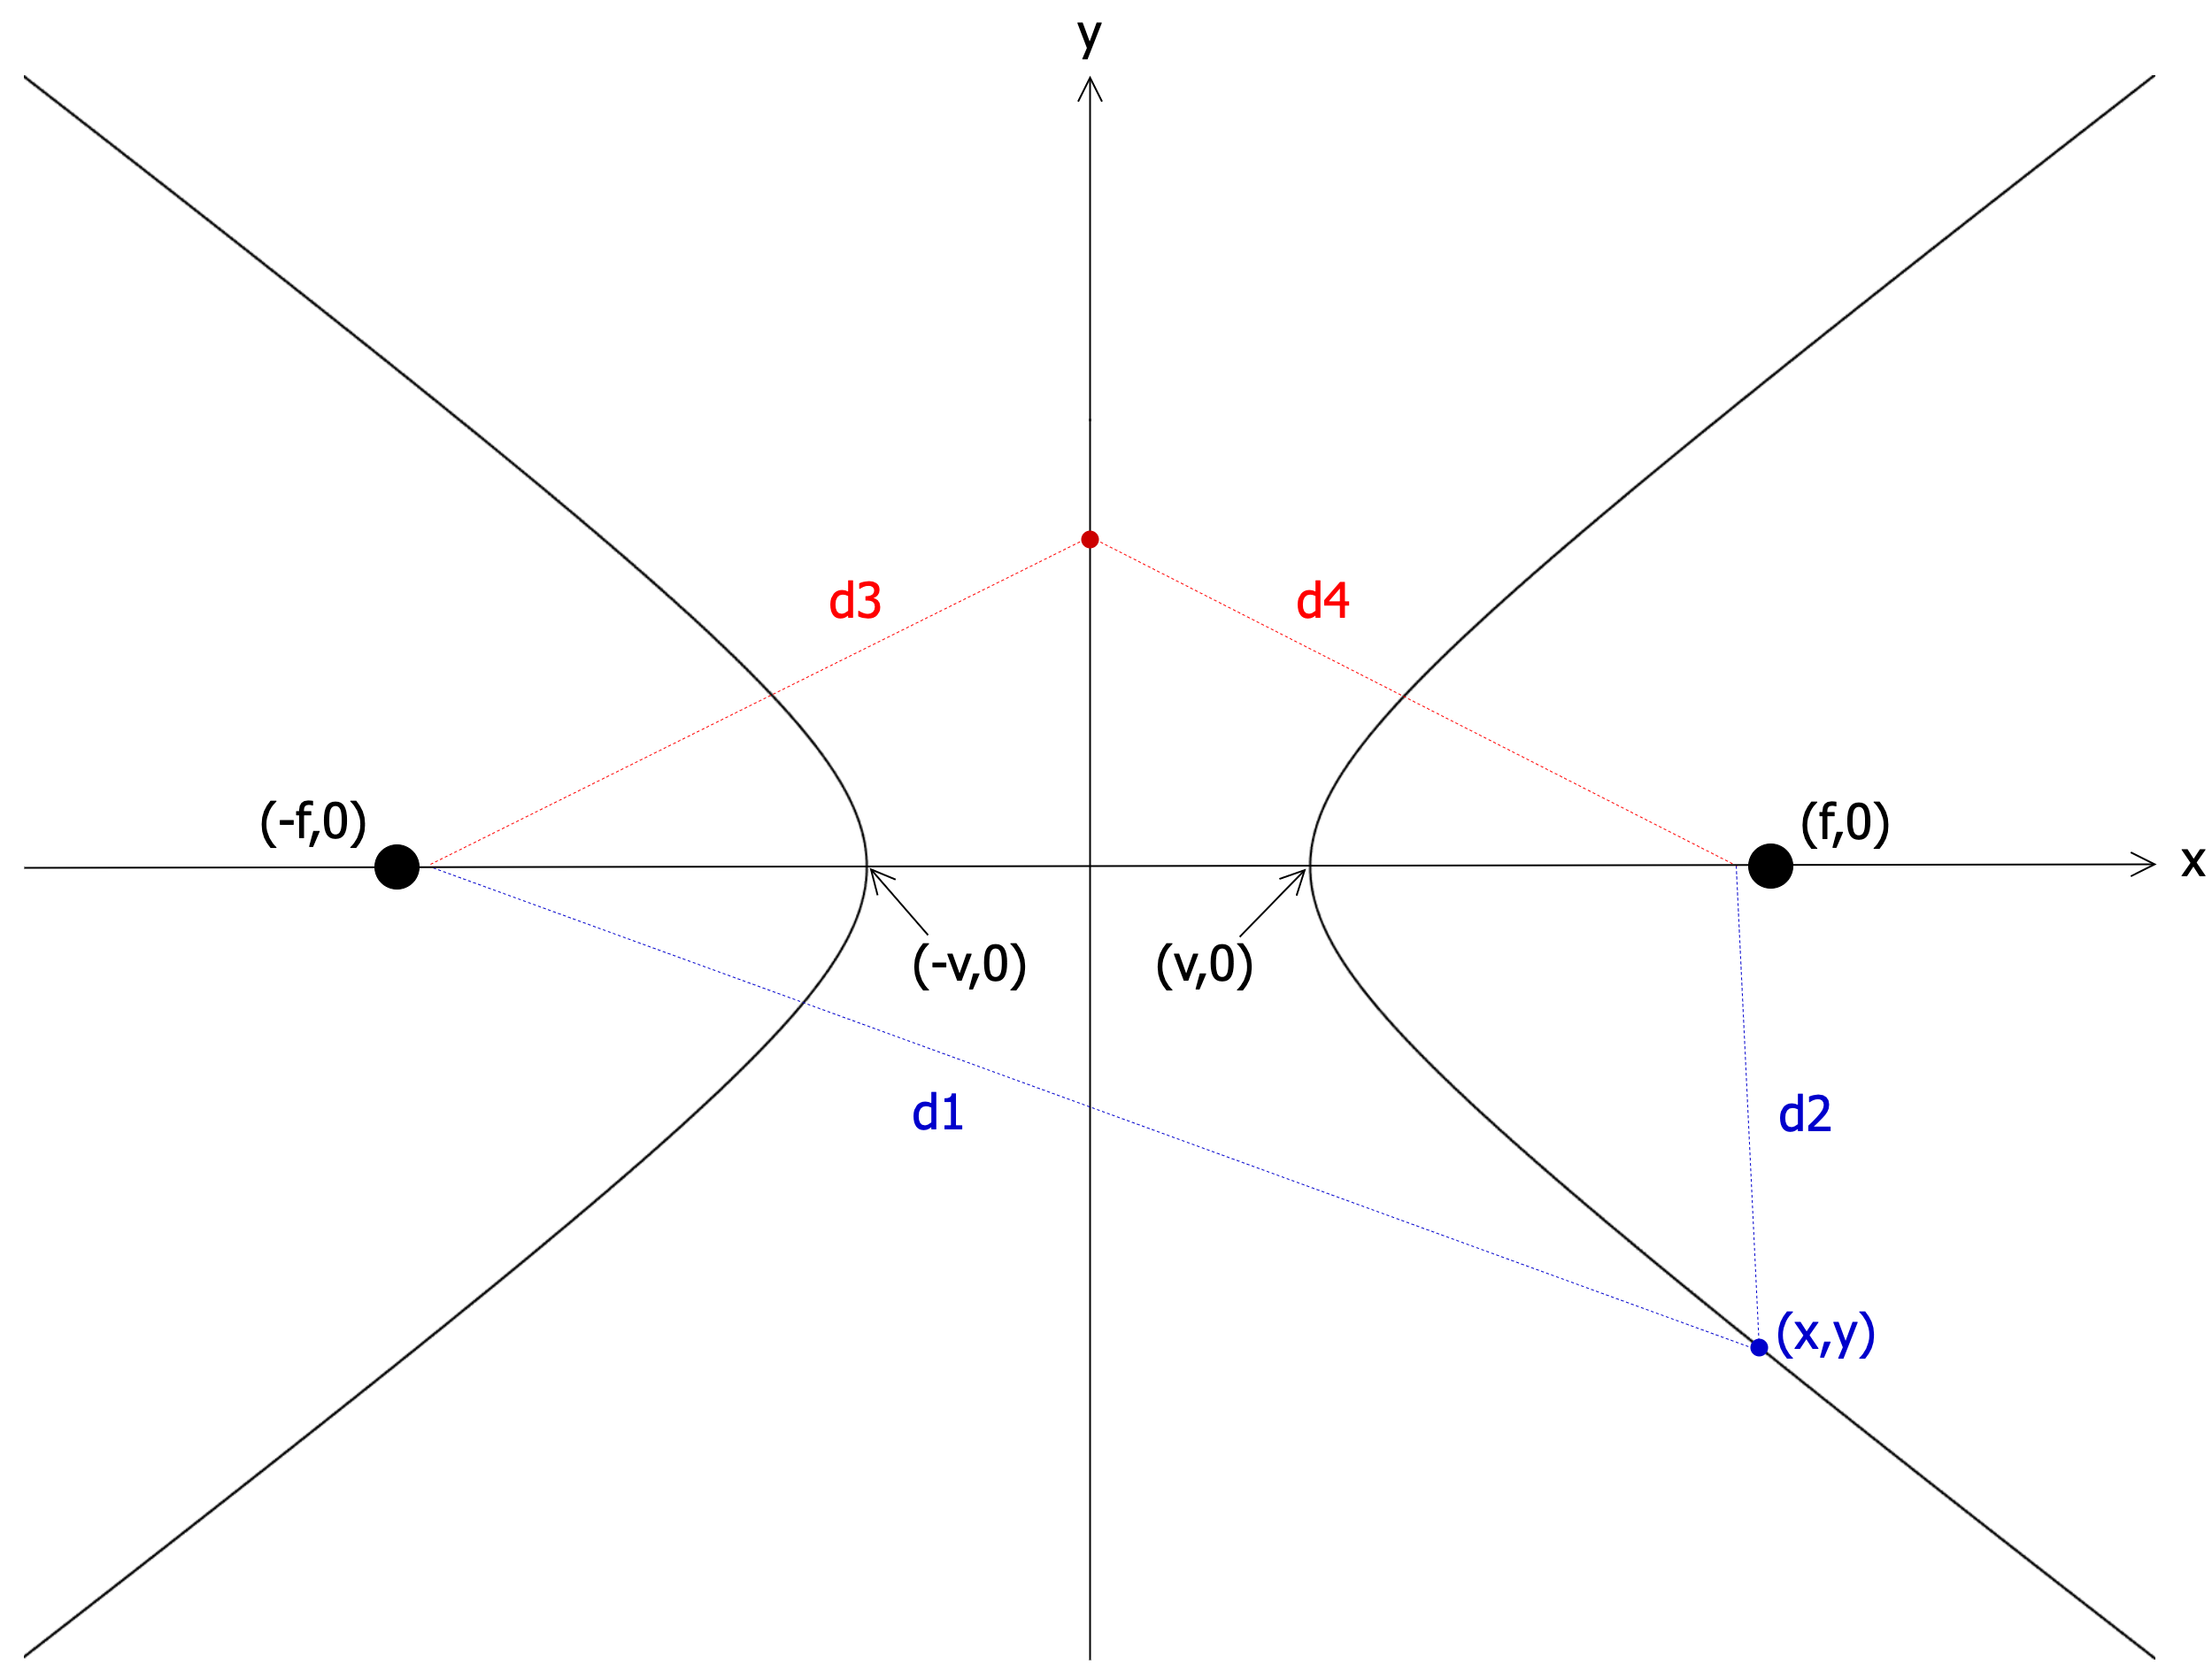
\includegraphics[width=0.8\textwidth]{figures/hyperbole-dist}
	\captionsetup{justification=centering,margin=2cm}
	\caption{Hyperbolic representation of acoustic source position possibilities in relation to ToA to two hydrophones}
	\label{fig:hyper}
\end{figure}

\subsubsection{ToA approximation}

In order to estimate the location of an acoustic source we take into account the phase differences between each pair of hydrophones, carefully explained in section \ref{subchap:HDL module}. These phase differences can be translated into periods of the signal which combined with the ToA obtained from correlation of arriving acoustic signals are equivalent to relative distances.

Following the previous idea, it is possible to model the distance of one sensor to the target based on the known distance of a second sensor to the same target. 
This is to say that for two sensors with known relative positions where hydrophone 1 is the closer to the target, the distance from hydrophone i to the target, $D_i$, can be expressed as the distance of hydrophone j to the target, $D_j$, added by the time difference of arrival, $\Delta t_{ij}$, multiplied by the propagation velocity, $c_s$. Overall, this relationship is declared in equation \ref{eq:dist_to_target}.

\begin{eqnarray}
& D_i = D_j + \Delta t_{ij} * c_s
\label{eq:dist_to_target}
\end{eqnarray}

Therefore, the same logic can be applied for multiple hydrophones. In the present work, in which it is considered a system with four hydrophones, a synchronization mechanism allows to determine the signals' ToA between the transceiver and the hydrophones. However, in order to simplify the synchronicity and decrease errors that arise from it, the module that precisely computes the phase differences of the received signal in the hydrophones is used so that is possible to apply the relationship in \ref{eq:dist_to_target}. Consequently, a better angle of arrival estimation can be achieved when using this approximation than if all four times of arrival are used for the same purpose.

\subsubsection{Doppler Effect}

The implemented process uses the information of the operating frequency of the transmitted signal in order to compute the phase differences and determine the overall times of arrival. However, the frequency is only completely stationary in a theoretical situation. In real scenarios, the environmental conditions and additional factors can change this frequency from the source to the receiver. In the present study, since the vehicle is predominantly moving then the Doppler effect could influence the signal's frequency, leading to erroneous calculations.

In order to evaluate if the Doppler effect influences the present system, it is possible to calculate which would be the frequency deviation observed for a known relative speed. Considering that the relative speed between the transmitter and the receiver takes a value of $relative\_speed$, using a fixed sound speed, $c_s$, and knowing the frequency of the transmitted signal, the relation \ref{eq:doppler} can be established. 

%\begin{eqnarray}
%&freq\_deviation = \frac{relative\_speed}{c_s} \times signal\_freq
%\label{eq:doppler}
%\end{eqnarray}

\note{desprezavel}
\note{frequency detector can be integrated}

\subsection{Methodological Approach} \label{subsec:estimator}

The goal of the proposed system is to estimate the position of an acoustic source in relation to known positions of a configuration of sensors, in a system of geometric axes with a defined origin. For this purpose, the logic employed is based on vector algebra with other physical considerations, detailed in the present subsection. 

Figure \ref{fig:AoA-init} represents the schematic of a considered scenario, where four hydrophones are placed in known relative positions in space and the origin of the axis is set on the body of the AUV or an alternative fixed structure. Then $r_i$ is defined as the vector that connects the origin of the axis to hydrophone $i$ and $rr_i$ defines the vector that connects hydrophone $i$ to the acoustic source. The black cross represents the acoustic source which is located somewhere in space. At last, the subtraction of the mentioned vectors is equal to $r$, according to \ref{eq:sum-vec}, which corresponds to the position of the acoustic source in relation to the origin of the axis and, overall, it is the variable that the method aims to determine.

\begin{eqnarray}
& r_i = r + rr_i
\label{eq:sum-vec}
\end{eqnarray}

\begin{figure}[!htbp]
	\centering
	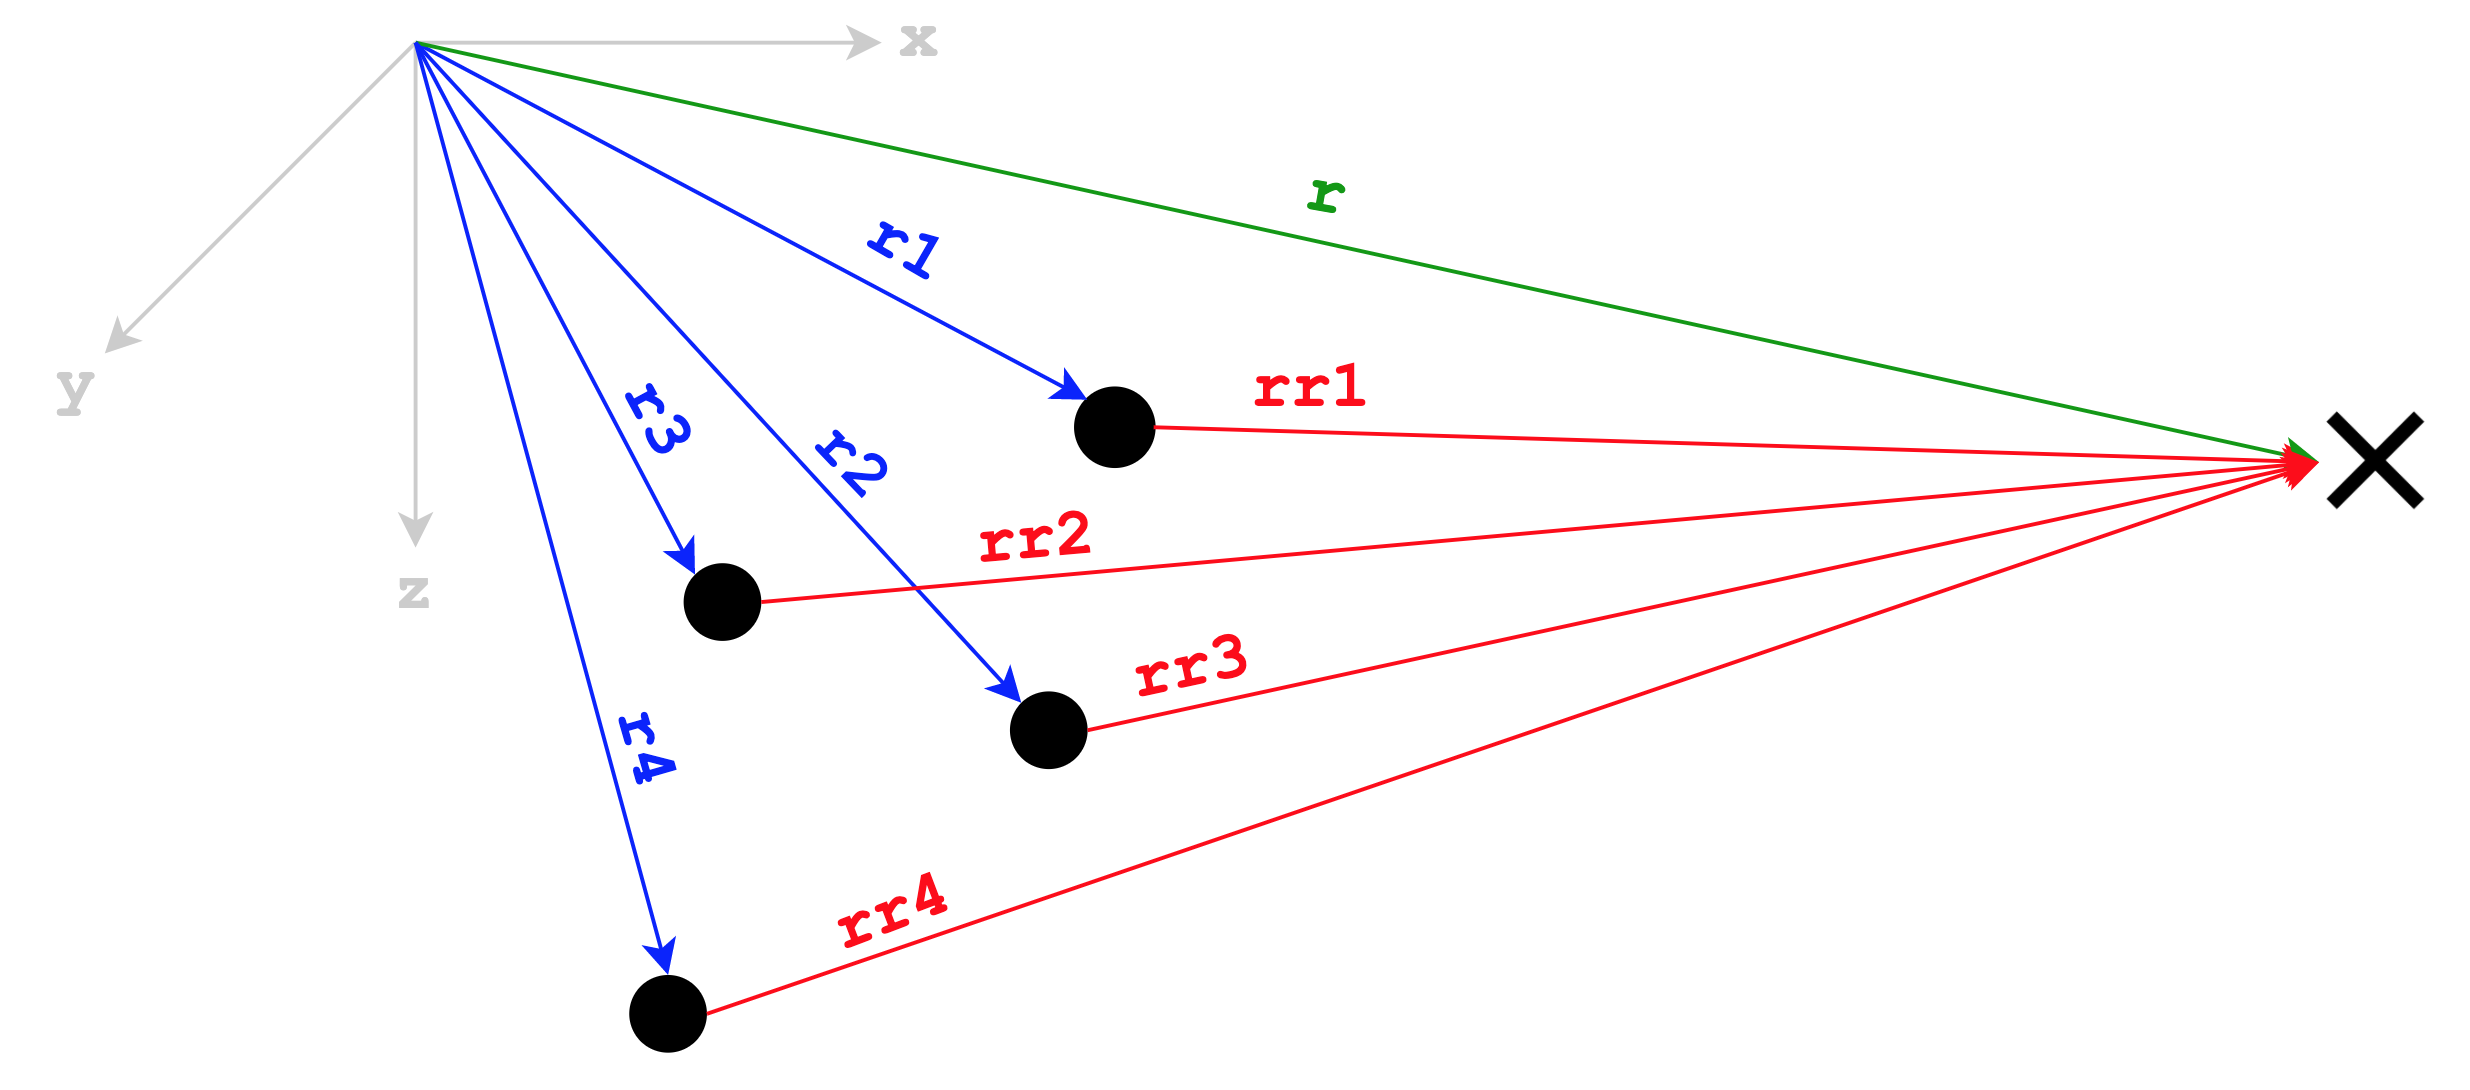
\includegraphics[width=0.8\textwidth]{figures/AoA-init}
	\captionsetup{justification=centering,margin=2cm}
	\caption{Considered scheme for angle of arrival estimation}
	\label{fig:AoA-init}
\end{figure}

Then we can define the times of arrival to each hydrophone as \ref{eq:toa-4h}, where $t_0$ is the absolute time of emission, $c_s$ is the underwater sound speed and $\rho_i$ is the norm of $rr_i$, \ref{eq:rho}, which translates to the distance from hydrophone $i$ to the acoustic source. 

\begin{eqnarray}
& t_i = t_0 +  \frac{\rho_i}{c_s}
\label{eq:toa-4h}
\end{eqnarray}

 However, as explained in the previous section, instead of using the absolute ToA in each hydrophone by computing the expression \ref{eq:toa-4h} for each of them, it can be expressed as a function of a single reference ToA. A simple logic was applied in order to determine this reference hydrophone, which starts by identifying the closest to the acoustic source. This allows to obtain all relative times of arrival by adding the defined reference time to each  between a hydrophone and the reference one. This is achieved by analyzing the  of each pair, $ \Delta t_{ij}$, for all possible combinations of two among four hydrophones, making up a total of six combinations. Considering each hydrophone pair $ij$ with $i, j= \{1,2,3,4\}$ :
 
 \begin{itemize}
 	\item if $ \Delta t_{ij}$ is positive, then hydrophone $i$ is closer to the acoustic source
 	\item if $ \Delta t_{ij}$ is negative, then hydrophone $j$ is closer to the acoustic source
 	\item if $ \Delta t_{ij}$ is zero, then $i$ and $j$ hydrophones are equidistant to the acoustic source
 \end{itemize}
 
Considering these relations, it is possible to compose a vector that accumulates the closer hydrophone between each pair for a certain position of the acoustic source. Extracting the mode of this vector will then return the chosen hydrophone in most cases and therefore the overall closer to the acoustic source. If the closer hydrophones are the equidistant to the source, then it is indifferent which one is selected.  

Thereafter, recalling expression \ref{eq:dist_to_target}, it is possible to write \ref{eq:toa_relation2}, \ref{eq:toa_relation3} and \ref{eq:toa_relation4} which translate the used relations, where  the chose reference sensor is hydrophone 1, for the purpose of exemplification.

\begin{eqnarray}
& T_2 = T_1 + \Delta t_{12} * c_s
\label{eq:toa_relation2}\\
& T_3 = T_1 + \Delta t_{13} * c_s
\label{eq:toa_relation3}\\
& T_4 = T_1 + \Delta t_{14} * c_s
\label{eq:toa_relation4}
\end{eqnarray}

If then the distance $\rho_i$ is raised to the power of two, we know that $||rr_i||^2 = r_i^{T}r_i$, which allows to deduce equation \ref{eq:rho1} after some mathematical manipulation. Considering $\rho_i$ a physical distance, it is also possible to express it trough equation \ref{eq:rho2}, which uses the speed of propagation underwater multiplied by the ToA of the signal from the acoustic source to hydrophone $i$.

\begin{eqnarray}
& \rho_i = ||rr_i|| 
\label{eq:rho}\\
&\rho_i^{2} =  r^{T}r + 2r^{T}r_i + r_i^{T}r_i
\label{eq:rho1}\\
&\rho_i^{2} = c_s^{2} (t_i-t_0)^{2}
\label{eq:rho2}
\end{eqnarray}

Since two distinct relations are defined for $\rho_i^{2}$, then it is possible to consider the algebraic expressions as equivalent, thus forming a single equation to be resolved with only one unknown variable. After some mathematical manipulation, the matrix relation \ref{eq:AoA-matrix} is achieved, where $r$ is isolated and can be estimated.

\begin{eqnarray}
\begin{bmatrix}
1 & 2\: r_i^{T}
\end{bmatrix}
\begin{bmatrix}
r^{T} r \\
r
\end{bmatrix}
=  
\begin{bmatrix}
c_s^{2} (t_i-t_0) - r_i^{T} r_i
\end{bmatrix}
\label{eq:AoA-matrix}
\end{eqnarray}
 
In order to resolve this system of equations and isolate $r$, the least squares method is applied. If \ref{eq:AoA-matrix} is extended to the four considered hydrophones, we obtain matrix $A$ represented as \ref{eq:A} and $Y$ equivalent to \ref{eq:Y}. It is important to notice that the $A$ matrix has to be invertible, thus the rows which contain the chosen hydrophone configuration have to be linearly independent. The least squares method is then expressed as \ref{eq:least-square}, where $X$, $\mathbb{R}^{4}$, holds the Cartesian result of $r$. As the method formulates four equations that are meant to calculate only three coordinates, $X$ will contain a fourth element that consists on a nonlinear component to $||r||^{2}$. This causes the estimator to be considered not efficient.

\begin{eqnarray}
& A = 
\begin{bmatrix}
1 & 2\: r_1^{T}\\
1 & 2\: r_2^{T}\\
1 & 2\: r_3^{T}\\
1 & 2\: r_4^{T}
\end{bmatrix}
\label{eq:A}
\end{eqnarray}

\begin{eqnarray}
& Y = 
\begin{bmatrix}
c_s^{2}\: (t_1-t_0)^2 - r_1^{T} r_1\\
c_s^{2}\: (t_2-t_0)^2 - r_2^{T} r_2\\
c_s^{2}\: (t_3-t_0)^2 - r_3^{T} r_3\\
c_s^{2}\: (t_4-t_0)^2 - r_4^{T} r_4\\
\end{bmatrix}
\label{eq:Y}
\end{eqnarray}

\begin{eqnarray}
& X = (A^{T}*A)^{-1}*A^{T}*Y
\label{eq:least-square}
\end{eqnarray}

After infer the Euclidean vector $r$, it is possible to obtain both the bearing trough its direction, $\hat{\boldsymbol{r}}$, and the range through its magnitude, $||r||$.

\subsection{Precision analysis}  \label{subchap:precision-analy}

\note{accuracy or precision?}
A methodology was formulated in order to evaluate the precision that the estimator can achieve in defined circumstances. For this initial approach to the study, the following conditions are considered: 

\begin{enumerate}[label=\alph*)]
	%--------------------
	\item \textbf{Sensor Configuration}  
	
	Each hydrophone configuration is analyzed individually. It is a parameter to be always defined and known from the begging of each simulation.
	
	%--------------------
	\item \textbf{Reference axis}
	
	 The origin of the reference axis is defined at the center of mass of the structure where the hydrophones are fixed, which in this case is the AUV.
	
	%--------------------
	\item \textbf{Injected error} 
	
	In order to make the study more realistic, an $e_i$ error is added to the time differences of arrival, $ \Delta t_{ij}$. These errors are mutually independent and follow a Gaussian distribution with zero mean and a configurable variance of $\sigma^{2}$, i.e., $e_i \sim \mathcal{N}(0,\,\sigma^{2})$. 
	
	 For the simulations performed in this project, a deviation of 5$^{\circ}$,or a window of $[-2.5^{\circ},2.5^{\circ}]$, in the angle of arrival estimation was considered to be reasonable for an underwater navigation scenario. Therefore, since the specified period of the signal is $T = \frac{1}{24400}$ and one period corresponds to a 360$^{\circ}$ phase shift, then the 5$^{\circ}$ will be equivalent to $\frac{5^{\circ}}{360^{\circ}}*T$ which is approximately a deviation of $0.5\mu s$. Hence the considered standard deviation $\sigma$ of the error $e_i$ in the computed time differences of arrival is equal to $0.5\mu s$.
	 
	 %--------------------
	 \item \textbf{Acoustic source position} 
	 
	 The considered positions for the acoustic source are defined in spherical coordinates. Thus the norm, $n$, corresponds to the source's range, whereas the azimuth, $\phi$, and elevation, $\theta$, define the angle of arrival of the received signal.
	 
	 Recalling the definition of spherical coordinates, it is known that for elevations of -90$^{\circ}$ or 90$^{\circ}$, the azimuth angle is meaningless and should not be considered. Since this system is affected by a Gaussian error, then the estimated azimuth angle is expected to return large errors not only for the absolute mentioned elevation values but for a considerable interval around it, dependent on the injected deviation. For that reason, the elevation values are limited to an interval between -80$^{\circ}$ and 80$^{\circ}$ so that the evaluated metrics present a result that is not so reflective of the errors originated from this phenomenon.
	 
	 The positions to be estimated are contained in a matrix with a number of columns equal to the number of positions and three rows consisting of its spherical coordinates. The matrix is arranged so that for each defined norm, the elevation component covers the interval [-80$^{\circ}$ to 80$^{\circ}$] in steps of one and, for each elevation value, the azimuth component covers the interval [-180$^{\circ}$, 180$^{\circ}$] in steps of one, forming partial spheres around the reference axis' origin.

	%--------------------
	\item \textbf{Propagation speed}
	
	In all performed simulations, the considered speed of sound is $1500 \; m/s$, which corresponds to the underwater propagation velocity of waves in typical conditions.
	
\end{enumerate}

Having the conditions enumerated, the logic of the algorithm occurs as follows. For every defined position of the acoustic source, $s$, a function that consists on the estimator is called, receiving as input the $s$, the positions of the hydrophone configuration, $r_i$, and an injected error in the . It then returns the estimated position of the source in Cartesian coordinates, $[x,y,z]$, and in spherical coordinates, $[n, \phi, \theta]$. As the position $s$ in Cartesian corresponds to the real value that is intended to be estimated, we can also obtain the real spherical coordinates by directly converting $s$ using the Cartesian to spherical relations in \ref{eq:cart2sph}.

\begin{eqnarray}
\begin{cases} 
n =  \sqrt{x^2 + y^2 + z^2}\\ 
\phi  = arctan \frac{y}{x}\\ 
\theta =  arctan \frac{\sqrt{x^2+y^2}}{z}
\end{cases}
\label{eq:cart2sph}
\end{eqnarray}

Consequently all conditions are met to analyze the achieved error in each coordinate by comparing the real position to the estimated values as \ref{eq:error1}, where the tested coordinates are $x, y, z, n, \phi$ and $\theta$.

\begin{eqnarray}
&error_{coordinate} = |estimated_{coordinate} - real_{coordinate}|
\label{eq:error1}
\end{eqnarray}

The metrics used to evaluate the quality of the estimator were :

\begin{itemize}
	\item \textbf{Mean squared error} (MSE): Incorporates both the variance and the bias of the estimator and indicates its overall quality
	\item \textbf{Standard deviation of the error} ($\sigma$) : Indicates how disperse are the estimates from the expected value
	\item \textbf{Minimum error ($min(e_i)$)} : Indicates the minimum error that is obtained by the estimator, thus the best absolute precision achieved
\end{itemize} 

\subsection{Simulations}

A series of simulations were performed in order to understand the behavior and capabilities of the estimator and analyze its overall precision.

To illustrate a scenario where this estimator is applicable, we can consider that a vehicle is moving towards an acoustic signal transmitter whose position is unknown. Imagining that the target is at a considerable distance, then the main focus is to achieve an optimal bearing estimation which provides a more direct path and saves resources. The range estimation serves as secondary measurement that indicates how near the vehicle is from the destination, so that it is possible to make control decisions such as moderate the navigation speed in the proximity of the target. For the reasons outlined, the study that follows presents a more thorough analysis of the azimuth and elevation errors. 

In this section, two different hydrophone configurations are considered, A and B defined in \ref{tab:configs_test1}, where the columns $r_{Ai}$ and $r_{Bi}$ contain the position's coordinates of each hydrophones $i$.

\begin{table}[!htbp] %use H to adjust
	\begin{center}
		\begin{tabular}{ l | c c c c | c c c c }
			%\hline
			%\multicolumn{1}{c|}{} & \multicolumn{4}{c|}{A} & \multicolumn{4}{c|}{B} \\
	    	\toprule
	       % \cline{2-9}
			\multicolumn{1}{c|}{} & $r_{A1}$ & $r_{A2}$ & $r_{A3}$ & $r_{A4}$ & $r_{B1}$ & $r_{B2}$ & $r_{B3}$ & $r_{B4}$ \\
			\midrule
			\multirow{1}{0.5em}{x} 
			& 0.02 & 0.02 & 0 & 0 & 0.1 & 0 & 0 & 0 \\
			%\hline 
			\multirow{1}{0.5em}{y} 
			& 0 & 0 & 0.1 & -0.1 & 0 & 0 & -0.0707 & 0.0707\\
			%\hline 
			\multirow{1}{0.5em}{z} 
			& 0.1 & -0.1  & 0 & 0 & 0 & 0.1 & -0.0707  & -0.0707\\
			\bottomrule 
		\end{tabular}
		\caption{Hydrophone configurations for precision tests}
		\label{tab:configs_test1}
	\end{center}
\end{table}

For the first simulation, configuration A is tested for the acoustic source positions previously described, in a total of 58121. The obtained plots are illustrated in \ref{fig:s1-A-n10}, where it is represented the error obtained by this specific configuration for all positions of the acoustic source.

\begin{figure}[!htbp]
	
	\makebox[\textwidth][c]{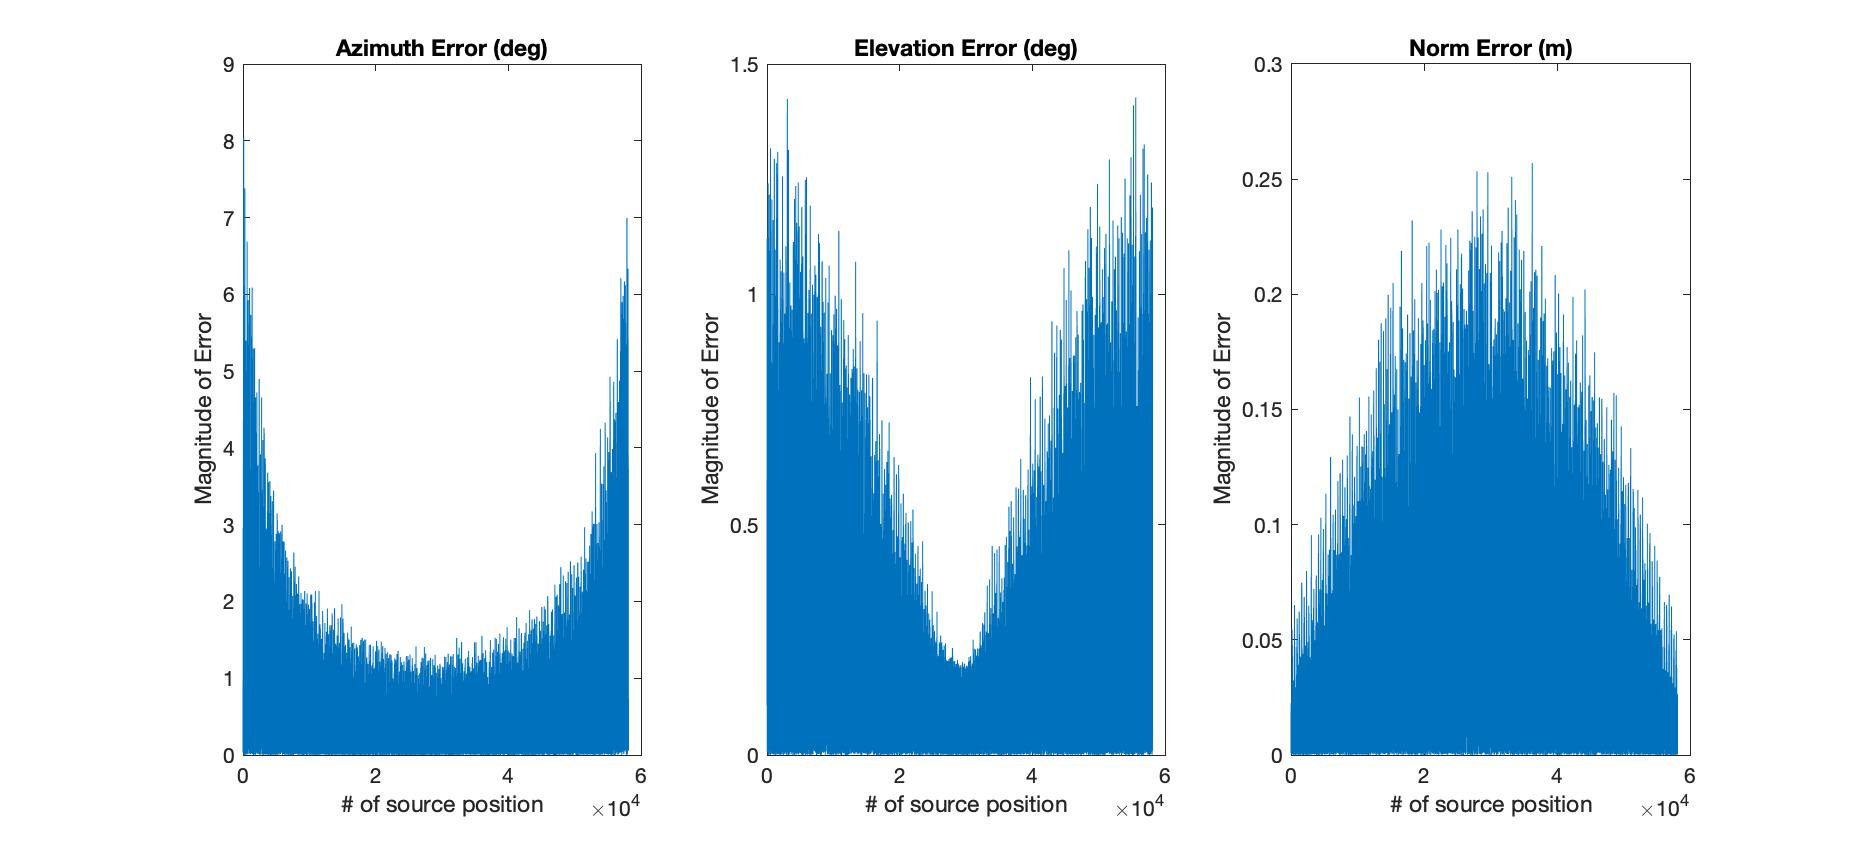
\includegraphics[width=1.2\textwidth]{figures/plots/plot-s1-A-n10}}
	\captionsetup{justification=centering,margin=2cm}
	\caption{Plots of azimuth, elevation and norm errors for defined source positions}
	\label{fig:s1-A-n10}
\end{figure}

Some conclusions can be drawn about configuration A from the obtained results :
\begin{itemize}
	\item A deviation in the estimate for positions with elevation close to its range limits causes:
	\begin{itemize}
				\item a higher azimuth error, since 
				\item a higher elevation error, since the configuration has a shorter baseline along the xx axis, between the pairs of hydrophone that are aligned in the yy and zz axis, then the elevation is more precisely estimated in positions that are approximated perpendicular line that passes in the middle of the configuration.
				
	\end{itemize}
	\item
\end{itemize}

\note{Add all conclusions}

Therefore, tables \ref{tab:azimuth-test1}  and \ref{tab:elevation-test1} illustrate the achieved results of azimuth error for several chosen norms.

\begin{table}[!htbp] %use H to adjust
	\begin{center}
		\begin{tabular}{ c | c c c c c }
			%\hline
			\toprule
			% \cline{2-9}
			\multicolumn{1}{c|}{Configuration} & Norm & MSE & Standard Deviation & Minimum \\
			\midrule
			\multirow{2}{*}{A} &10 & 0.5440 & 0.6050 & 8.7434$\times10^{-7}$\\
		%	&100 & 0.5465 & 0.6090 & 6.0529$\times10^{-6}$\\
			&1000 & 0.5425 & 0.5992 &  8.3781$\times10^{-6}$\\
			\midrule			
			\multirow{2}{*}{B} &10 & 0.2300 & 0.2129 & 1.3049$\times10^{-5}$\\
		%	&100 & 0.2304 & 0.2119  & 4.3874$\times10^{-6}$\\
			&1000 & 0.2230 & 0.2115 & 4.0963$\times10^{-6}$\\
			\bottomrule 
		\end{tabular}
		\caption{Comparison of obtained azimuth errors for different configurations}
		\label{tab:azimuth-test1}
	\end{center}
\end{table}

\begin{table}[!htbp] %use H to adjust
	\begin{center}
		\begin{tabular}{ c | c c c c c }
			%\hline
			\toprule
			% \cline{2-9}
			\multicolumn{1}{c|}{Configuration} & Norm & MSE & Standard Deviation & Minimum \\
			\midrule
			\multirow{2}{*}{A} &10 & 0.5440  & 0.1856 & 3.1025$\times10^{-6}$  & \\
		%	&100 & 0.5465 &  0.1845 &  2.1818$\times10^{-6}$ & \\
			&1000 & 0.5425 & 0.1854 & 5.0595$\times10^{-6}$ & \\
			\midrule			
			\multirow{2}{*}{B} &10 & 0.2300 & 0.0668 & 2.7903$\times10^{-5}$ \\
		%	&100 & 0.2304 & 0.0662 & 1.0184$\times10^{-5}$\\
			&1000 & 0.2230 & 0.0663 & 4.3935$\times10^{-6}$ \\
			\bottomrule 
		\end{tabular}
		\caption{Comparison of obtained elevation errors for different configurations}
		\label{tab:elevation-test1}
	\end{center}
\end{table}


\subsubsection{Influence of quantization on precision}

The first term to be analyzed is how much does the quantization of the calculations influence the obtained precision of the estimator. In order to analyze this, a simple adaptation was made to the numeric precision of the  values that are input of the system. Instead of using the MATLAB precision of fifteen decimal places, the value was truncated to a specified number of decimal places, $\kappa$.
Since the time differences of arrival have magnitudes around microseconds, then initially the time differences of arrival are multiplied by $10^6$ to avoid missing information. Then the relation \ref{eq:trucate} is applied resulting in a truncated value of  with $\kappa$ decimal places.

\begin{eqnarray}
&_{truncated} = \frac{round(*2^{\kappa})}{2^{\kappa}};
\label{eq:trucate}
\end{eqnarray}

Finally after the truncation, the value is converted again to seconds to be used in the algorithm.

\note{Dar um exemplo de erro antes e erro depois da truncação}

\subsubsection{Influence of ToA measurement on position estimation}

 \note{ por simulação, conclui que para distancias muito longe (quantizar) não faz diferença ter o TOA e basta os TDOA}

\subsubsection{Influence of displacing a specific hydrophone}

The goal of this test is to understand what is the influence of moving one hydrophone along a certain direction in the overall error.

\note{-considerar uma configuração\\
- analysar evolução do erro\\
-concluir que aumentar baseline é melhor até o erro manter-se constante}

\subsection{Conclusions}

%Since this analysis is incident on a specific configuration, not all observations are generalizable.
However there are conclusions that can be taken from the inspection of multiple configurations, such as : 
\begin{itemize}
	\item incresed baseline (até certo ponto) outputs best results ; when baseline for a specific hydrophone or pair is too large, then it will decrease the angle vision for the shorter baselines
	\item the higher the range, the bigger the errors
	\item in higher ranges, the small angle variations can still indicate a big deviation of estimation from the original point in Cartesian coordinates
\end{itemize}

\note{- tenho sistema que estima os MSE, erro de azimute e elevação, para certas configuração consegue-se perceber padroes nos erros (e.g. erro aumenta com afastamento da source -> ao longe variações pequenas de angulo podem indicar deslocação da estimação grande )}

\note{escrever conclusoes gerais}
